\documentclass[a4paper,11pt]{article}

% ============================================
% PACKAGES
% ============================================
\usepackage[utf8]{inputenc}
\usepackage[T1]{fontenc}
\usepackage{fontspec}
\setmainfont{Arial}[Scale=1.0]
\usepackage[top=2cm, bottom=2cm, left=2cm, right=2cm]{geometry}
\usepackage{setspace}
\onehalfspacing
\usepackage{microtype}
\usepackage{parskip}
\setlength{\parskip}{6pt}
\setlength{\parindent}{0pt}
\usepackage{fancyhdr}
\pagestyle{fancy}
\fancyhf{}
\fancyfoot[C]{\thepage}
\renewcommand{\headrulewidth}{0pt}
\renewcommand{\footrulewidth}{0pt}
\usepackage{footmisc}
\renewcommand{\footnotelayout}{\fontsize{10}{12}\selectfont}
\usepackage{titlesec}
\titleformat{\section}{\fontsize{12}{14}\bfseries\selectfont}{\thesection}{1em}{}
\titleformat{\subsection}{\fontsize{12}{14}\bfseries\selectfont}{\thesubsection}{1em}{}
\titleformat{\subsubsection}{\fontsize{12}{14}\bfseries\selectfont}{\thesubsubsection}{1em}{}
\setcounter{secnumdepth}{3}
\setcounter{tocdepth}{3}
\usepackage{titling}
\usepackage{graphicx}
\usepackage{booktabs}
\usepackage{array}
\usepackage{multirow}
\usepackage{float}
\usepackage{amsmath}
\usepackage{listings}
\usepackage{xcolor}
\usepackage{tikz}
\usepackage{subcaption}
\usepackage[backend=biber,style=apa,apamaxprtauth=99]{biblatex}
\addbibresource{references.bib}

\lstset{
  language=Python,
  basicstyle=\ttfamily\small,
  commentstyle=\color{gray},
  stringstyle=\color{red},
  numbers=left,
  numberstyle=\tiny,
  numbersep=5pt,
  frame=single,
  breaklines=true,
  showstringspaces=false
}

% ============================================
% DOCUMENT INFORMATION
% ============================================
\newcommand{\thesistitle}{Comparative Analysis of CNN and Random Forest for Fashion-MNIST Classification}
\newcommand{\thesistype}{Research Report}
\newcommand{\coursename}{Machine Learning}
\newcommand{\courseofstudy}{Computer Science}
\newcommand{\thesisdate}{January 2026}
\newcommand{\authorname}{Student Name}
\newcommand{\matriculationnumber}{123456789}
\newcommand{\tutorname}{Tutor Name}

\begin{document}

% ============================================
% TITLE PAGE
% ============================================
\begin{titlepage}
	\centering
	\vspace*{2cm}
	{\fontsize{12}{14}\selectfont\bfseries\thesistitle}
	\vspace{2cm}
	{\fontsize{11}{13}\selectfont\thesistype}
	\vspace{2cm}
	{\fontsize{11}{13}\selectfont
		Course: \coursename\\[0.5cm]
		Course of Study: \courseofstudy
	}
	\vfill
	{\fontsize{11}{13}\selectfont
		\textbf{Author:} \authorname\\[0.3cm]
		\textbf{Matriculation Number:} \matriculationnumber\\[0.3cm]
		\textbf{Tutor:} \tutorname\\[0.3cm]
		\textbf{Date:} \thesisdate
	}
	\vspace{2cm}
\end{titlepage}

% ============================================
% FRONT MATTER
% ============================================
\pagenumbering{Roman}
\setcounter{page}{2}
\tableofcontents
\newpage

% ============================================
% MAIN TEXT
% ============================================
\pagenumbering{arabic}
\setcounter{page}{1}

\section*{Abstract}

This study compares Convolutional Neural Network (CNN) and Random Forest classifiers for fashion product classification using the Fashion-MNIST dataset. The CNN (MCNN15 architecture) achieved 93.63\% test accuracy compared to 87.52\% for Random Forest. Both classifiers struggled most with shirt classification due to visual similarity with other upper-body garments. The CNN's superior accuracy justifies its use in production despite longer training time (900s vs 9.45s).

\begin{figure}[H]
	\centering
	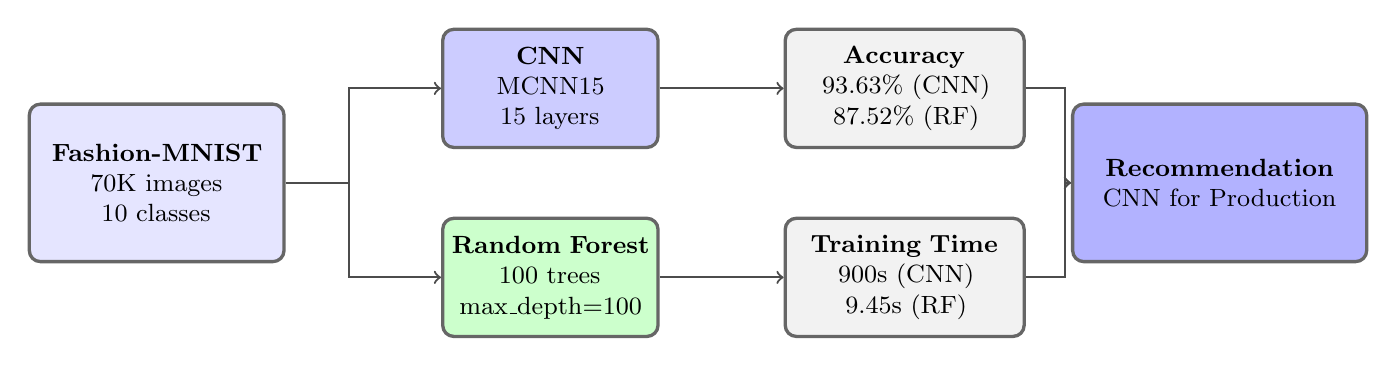
\begin{tikzpicture}[
			box/.style={rectangle, rounded corners, draw=black!60, very thick, minimum height=1.5cm, text centered, font=\small},
			dataset/.style={box, fill=blue!10, text width=3.0cm, minimum height=2cm},
			cnn/.style={box, fill=blue!20, text width=2.5cm},
			rf/.style={box, fill=green!20, text width=2.5cm},
			result/.style={box, fill=gray!10, text width=2.8cm},
			rec/.style={box, fill=blue!30, text width=3.5cm, minimum height=2cm},
			arrow/.style={->, thick, black!70}
		]

		% Dataset
		\node[dataset] (data) at (0,0) {\textbf{Fashion-MNIST}\linebreak 70K images\linebreak 10 classes};

		% Models with more spacing from dataset
		\node[cnn] (cnn) at (5,1.2) {\textbf{CNN}\linebreak MCNN15\linebreak 15 layers};
		\node[rf] (rf) at (5,-1.2) {\textbf{Random Forest}\linebreak 100 trees\linebreak max\_depth=100};

		% Results with more spacing
		\node[result] (acc) at (9.5,1.2) {\textbf{Accuracy}\linebreak 93.63\% (CNN)\linebreak 87.52\% (RF)};
		\node[result] (time) at (9.5,-1.2) {\textbf{Training Time}\linebreak 900s (CNN)\linebreak 9.45s (RF)};

		% Conclusion
		\node[rec] (rec) at (13.5,0) {\textbf{Recommendation}\linebreak CNN for Production};

		% Arrows with better spacing
		\draw[arrow] (data.east) -- ++(0.8,0) |- (cnn.west);
		\draw[arrow] (data.east) -- ++(0.8,0) |- (rf.west);
		\draw[arrow] (cnn.east) -- ++(0.6,0) |- (acc.west);
		\draw[arrow] (rf.east) -- ++(0.6,0) |- (time.west);
		\draw[arrow] (acc.east) -- ++(0.5,0) |- (rec.west);
		\draw[arrow] (time.east) -- ++(0.5,0) |- (rec.west);

	\end{tikzpicture}
	\caption{Graphical Abstract: Comparative analysis workflow from Fashion-MNIST dataset through CNN and Random Forest classifiers to performance metrics and production recommendation.}
	\label{fig:graphical_abstract}
\end{figure}

\section{Introduction}

The fashion retail industry requires automated product classification for inventory management and visual search applications. While Convolutional Neural Networks (CNNs) demonstrate strong performance on fashion classification, traditional methods such as Random Forest remain relevant due to faster training times, interpretability, and lower computational requirements.

Prior work on Fashion-MNIST focuses primarily on maximizing accuracy through increasingly complex architectures, without addressing practical trade-offs that influence production deployment decisions. Production systems must balance accuracy against training time, model size, and inference latency.

This study addresses this gap by comparing MCNN15 \parencite{bhatnagar2017}, a 15-layer CNN optimized for Fashion-MNIST, against the optimal Random Forest configuration \parencite{xiao2017}. These classifiers are evaluated across accuracy, per-category metrics, confusion patterns, training times, and model sizes to provide evidence-based recommendations for production systems.

Section 2 reviews CNN architectures and benchmarking studies. Section 3 describes the Fashion-MNIST dataset. Section 4 outlines methodology. Sections 5 and 6 present results and analysis, followed by conclusions in Section 7.

\section{Literature Review}

\subsection{Evolution of CNN Architectures for Image Classification}

CNN development has progressed from \textcite{lecun1998}'s LeNet-5 through \textcite{krizhevsky2012}'s AlexNet to modern deep architectures. \textcite{simonyan2014}'s VGG demonstrated that small 3$\times$3 filters stacked deeply (16-19 layers) achieve superior performance, while \textcite{he2016}'s ResNet introduced skip connections enabling networks exceeding 100 layers. These advances established the foundational patterns---convolutional feature extraction, progressive depth, and residual learning---that underpin contemporary computer vision.

\subsection{Fashion-MNIST Benchmarking Studies}

Since its introduction by \textcite{xiao2017}, Fashion-MNIST has become a standard benchmark with CNN accuracies ranging from 90\% to 99\% \parencite{mukhamediev2024}. Simple 4-6 layer CNNs achieve 91-93\% accuracy, while deeper architectures reach 96-99\%. \textcite{bbouzidi2024} demonstrated that CNNs remain competitive against Vision Transformers on this dataset due to their inductive biases for local features. \textcite{cavallo2022} established that moderate-depth networks (15-20 layers) offer optimal accuracy-efficiency trade-offs, informing architecture selection for this study.

\subsection{CNN vs Traditional Machine Learning for Image Classification}

CNNs automatically learn hierarchical spatial features from raw pixels, whereas traditional methods like Random Forest require flattened vectors and manual feature engineering. \textcite{xiao2017} demonstrated this performance gap on Fashion-MNIST: Random Forest achieved 87.5\% accuracy versus 91\% for shallow CNNs. CNNs preserve spatial relationships through convolution and achieve translation invariance via pooling, while flattening destroys two-dimensional structure. \textcite{sathyadevan2015} noted that although Random Forest trains faster (seconds vs. minutes), CNNs' superior generalization justifies their use in production systems where accuracy impacts revenue.

\subsection{Selection of MCNN15 Architecture}

MCNN15 \parencite{bhatnagar2017} was selected for four reasons: (1) native Fashion-MNIST optimization without input modification, (2) optimal depth-efficiency balance with 15 layers and batch normalization \parencite{ioffe2015} that achieves 93.6\% accuracy without overfitting, (3) group-wise architecture with progressive channel expansion (32$\rightarrow$64$\rightarrow$256) capturing multi-scale features from textures to garment shapes, and (4) documented performance providing a clear benchmark for Random Forest comparison. Unlike VGG-16 or ResNet-50, MCNN15 offers competitive accuracy with lower computational requirements on this relatively small dataset.

\section{Dataset Description}

\subsection{Origin and Motivation}

Fashion-MNIST was introduced by Zalando Research in 2017 as a modern replacement for MNIST, which had become too easy for contemporary deep learning (CNNs now achieve $>$99.7\% accuracy) \parencite{xiao2017}. This dataset provides a more challenging benchmark for fashion product classification in e-commerce applications including automated inventory management and visual search.

\subsection{Dataset Statistics}

Fashion-MNIST comprises 70,000 grayscale images at 28$\times$28 resolution, divided into 60,000 training and 10,000 test samples. This format serves as a drop-in MNIST replacement while providing greater classification challenge. The grayscale format and compact resolution balance computational efficiency with sufficient visual detail for accurate garment classification.

\subsection{Class Distribution}

The dataset contains 10 balanced fashion categories with exactly 6,000 training and 1,000 test samples per class. This balanced distribution eliminates the need for class weighting or specialized sampling techniques, enabling straightforward comparison between classifiers.

\subsection{Class Labels and Examples}

Table \ref{tab:classes} presents the complete list of Fashion-MNIST categories with class indices and representative characteristics.

\begin{table}[H]
	\centering
	\caption{Fashion-MNIST Class Labels and Descriptions}
	\label{tab:classes}
	\begin{tabular}{|c|l|l|}
		\hline
		\textbf{Index} & \textbf{Label} & \textbf{Description}                      \\
		\hline
		0              & T-shirt/top    & Short-sleeved upper body garments         \\
		1              & Trouser        & Long pants covering both legs             \\
		2              & Pullover       & Knitted upper body garments               \\
		3              & Dress          & One-piece garment covering torso and legs \\
		4              & Coat           & Outerwear worn over other clothing        \\
		5              & Sandal         & Open footwear with straps                 \\
		6              & Shirt          & Buttoned upper body garments              \\
		7              & Sneaker        & Athletic footwear                         \\
		8              & Bag            & Hand-carried containers                   \\
		9              & Ankle boot     & Footwear covering ankle                   \\
		\hline
	\end{tabular}
\end{table}

Figure \ref{fig:dataset_samples} illustrates representative samples demonstrating the visual diversity, intra-class variability (e.g., different shirt styles), and inter-class similarities (e.g., shirts vs. T-shirts) that distinguish Fashion-MNIST from digit recognition.

\begin{figure}[H]
	\centering
	\includegraphics[width=\textwidth]{../../plots/dataset/samples.png}
	\caption{Representative samples from the Fashion-MNIST dataset showing five examples from each of the 10 fashion categories. The images demonstrate significant intra-class variability (e.g., different shirt styles) and inter-class similarity (e.g., shirts vs. T-shirts), making classification more challenging than handwritten digit recognition.}
	\label{fig:dataset_samples}
\end{figure}



\section{Methodology}

\subsection{Dataset and Preprocessing}

Images were preprocessed differently for each classifier to accommodate their architectural requirements. For the Random Forest classifier, the 28$\times$28 pixel images were flattened into 784-dimensional feature vectors, treating each pixel as an independent feature. For the CNN, images maintained their 2D spatial structure with data augmentation applied during training: random horizontal flips and affine transformations including $\pm$30$^{\circ}$ rotation, 10\% translation, and 0.9-1.1 scaling factors. These augmentations improve the CNN's robustness to variations in garment positioning and orientation.

\subsection{Random Forest Classifier}

Following \textcite{xiao2017}, the implementation uses scikit-learn with: n\_estimators=100, max\_depth=100, criterion=entropy, n\_jobs=-1. This configuration balances model complexity with generalization.

\subsection{CNN Architecture (MCNN15)}

The MCNN15 architecture \parencite{bhatnagar2017} comprises 15 convolutional layers organized into three groups with batch normalization \parencite{ioffe2015} and max pooling, followed by fully connected layers (288$\rightarrow$32$\rightarrow$10). Figure \ref{fig:mcnn15_arch} illustrates the architecture.

\begin{figure}[H]
	\centering
	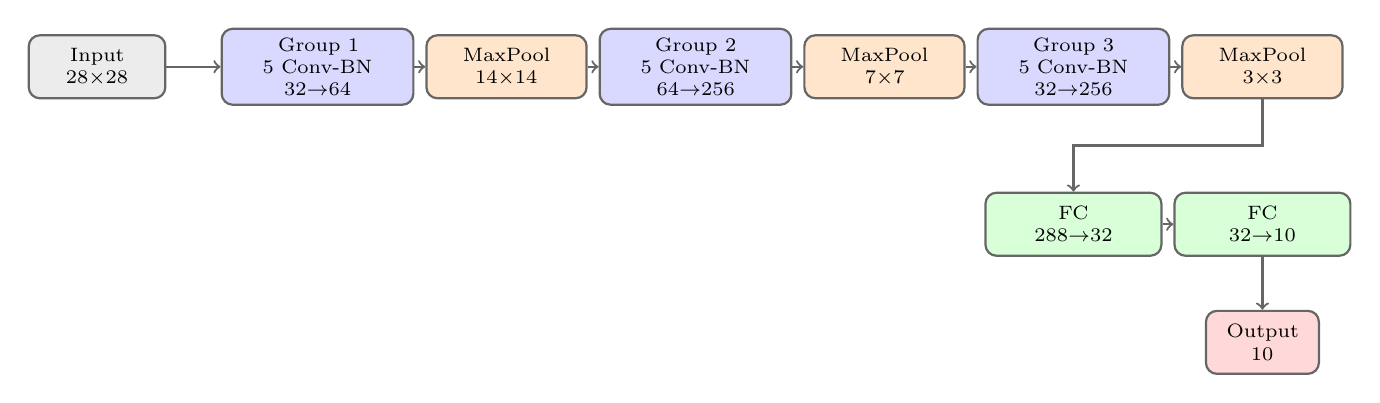
\begin{tikzpicture}[
			box/.style={rectangle, rounded corners, draw=black!60, thick, minimum height=0.8cm, text centered, font=\scriptsize},
			conv/.style={box, fill=blue!15, text width=2.2cm},
			pool/.style={box, fill=orange!20, text width=1.8cm},
			fc/.style={box, fill=green!15, text width=2cm},
			arrow/.style={->, thick, black!60},
			label/.style={font=\tiny\bfseries}
		]

		% Input
		\node[box, fill=gray!15, text width=1.5cm] (input) at (0,0) {Input\\28$\times$28};

		% Group 1
		\node[conv] (g1) at (2.8,0) {Group 1\\5 Conv-BN\\32$\rightarrow$64};
		\node[pool] (p1) at (5.2,0) {MaxPool\\14$\times$14};

		% Group 2
		\node[conv] (g2) at (7.6,0) {Group 2\\5 Conv-BN\\64$\rightarrow$256};
		\node[pool] (p2) at (10,0) {MaxPool\\7$\times$7};

		% Group 3
		\node[conv] (g3) at (12.4,0) {Group 3\\5 Conv-BN\\32$\rightarrow$256};
		\node[pool] (p3) at (14.8,0) {MaxPool\\3$\times$3};

		% Classifier
		\node[fc] (fc1) at (12.4,-2) {FC\\288$\rightarrow$32};
		\node[fc] (fc2) at (14.8,-2) {FC\\32$\rightarrow$10};
		\node[box, fill=red!15, text width=1.2cm] (out) at (14.8,-3.5) {Output\\10};

		% Arrows
		\draw[arrow] (input) -- (g1);
		\draw[arrow] (g1) -- (p1);
		\draw[arrow] (p1) -- (g2);
		\draw[arrow] (g2) -- (p2);
		\draw[arrow] (p2) -- (g3);
		\draw[arrow] (g3) -- (p3);
		\draw[arrow] (p3) -- ++(0,-1) -| (fc1);
		\draw[arrow] (fc1) -- (fc2);
		\draw[arrow] (fc2) -- (out);

	\end{tikzpicture}
	\caption{MCNN15 architecture diagram showing the three convolutional groups with batch normalization and max pooling, followed by fully connected classifier layers. Each group contains 5 Conv-BN-ReLU blocks with progressive channel expansion.}
	\label{fig:mcnn15_arch}
\end{figure}

\subsection{Training Strategy}



\subsubsection{Random Forest Training}

Random Forest training used the complete 60,000-sample training set flattened to 784-dimensional vectors. No data augmentation was applied. Training completed in approximately 9.45 seconds using CPU parallelization.

\subsubsection{CNN Training}

The CNN was trained using Adam optimizer \parencite{kingma2014} with cross-entropy loss, learning rate=1e-3, weight decay=1e-5, and batch size=128 for 50 epochs. The training set was split 50,000/10,000 for training/validation. Data augmentation included random horizontal flips, rotation ($\pm$30$^{\circ}$), translation (10\%), and scaling (0.9-1.1). The best validation accuracy (93.74\%) was achieved at epoch 40. Training time: approximately 900 seconds on GPU. The procedure followed \textcite{bhatnagar2017} methodology.

\section{Results}

\subsection{Overall Performance}

Table \ref{tab:overall} presents comprehensive performance metrics for both classifiers on train and test sets.

\begin{table}[H]
	\centering
	\caption{Overall Performance Comparison}
	\label{tab:overall}
	\begin{tabular}{|l|c|c|c|c|}
		\hline
		\textbf{Metric} & \textbf{RF Train} & \textbf{RF Test} & \textbf{CNN Train} & \textbf{CNN Test} \\
		\hline
		Accuracy        & 100.00\%          & 87.52\%          & 95.47\%            & 93.63\%           \\
		Precision       & 100.00\%          & 87.42\%          & 95.49\%            & 93.63\%           \\
		Recall          & 100.00\%          & 87.52\%          & 95.47\%            & 93.63\%           \\
		Training Time   & 9.45s             & ---              & 900s               & ---               \\
		\hline
	\end{tabular}
\end{table}

The CNN achieved 6.11 percentage points higher test accuracy (48.8\% error reduction). Random Forest shows perfect training accuracy (100\%) but 12.48\% test error, indicating severe overfitting. The CNN demonstrates better generalization with only 1.84\% train-test gap.

\subsection{CNN Training Progression}

\begin{minipage}[t]{0.48\textwidth}
	Figure \ref{fig:cnn_training} shows CNN accuracy progression from 74.5\% (epoch 1) to 93.7\% (epoch 50). Validation (orange) and test (green) curves track closely with training (blue), indicating minimal overfitting. Validation peaks at epoch 41 (93.74\%). Rapid improvement (epochs 0-10) captures coarse features; the plateau (10-50) refines patterns for challenging categories.
\end{minipage}
\hfill
\begin{minipage}[t]{0.48\textwidth}
	\begin{figure}[H]
		\centering
		\includegraphics[width=\textwidth]{../../plots/cnn/training.png}
		\caption{CNN training curves over 50 epochs.}
		\label{fig:cnn_training}
	\end{figure}
\end{minipage}

\subsection{Per-Category Performance}

Table \ref{tab:percategory} details precision and recall by category.

\begin{table}[H]
	\centering
	\caption{Per-Category Precision and Recall}
	\label{tab:percategory}
	\resizebox{\textwidth}{!}{%
		\begin{tabular}{|l|c|c|c|c|c|c|c|c|}
			\hline
			                                    & \multicolumn{4}{c|}{\textbf{Random forest}} & \multicolumn{4}{c|}{\textbf{Convolutional Neural Network}}                                                                                                                                                    \\
			\cline{2-9}
			\multirow{-2}{*}{\textbf{Category}} & \multicolumn{2}{c|}{\textbf{Precision}}     & \multicolumn{2}{c|}{\textbf{Recall}}                       & \multicolumn{2}{c|}{\textbf{Precision}} & \multicolumn{2}{c|}{\textbf{Recall}}                                                                   \\
			\cline{2-9}
			                                    & \textbf{Train}                              & \textbf{Test}                                              & \textbf{Train}                          & \textbf{Test}                        & \textbf{Train} & \textbf{Test} & \textbf{Train} & \textbf{Test} \\
			\hline
			T-shirt/top                         & 99.8\%                                      & 81.3\%                                                     & 99.7\%                                  & 86.3\%                               & 95.1\%         & 86.7\%        & 94.8\%         & 89.2\%        \\
			Trouser                             & 100.0\%                                     & 99.3\%                                                     & 100.0\%                                 & 95.9\%                               & 99.8\%         & 99.2\%        & 99.6\%         & 98.5\%        \\
			Pullover                            & 99.9\%                                      & 76.6\%                                                     & 99.8\%                                  & 79.5\%                               & 96.8\%         & 90.5\%        & 96.2\%         & 89.3\%        \\
			Dress                               & 99.9\%                                      & 87.3\%                                                     & 99.9\%                                  & 90.9\%                               & 96.5\%         & 91.8\%        & 96.8\%         & 93.5\%        \\
			Coat                                & 99.9\%                                      & 76.1\%                                                     & 99.8\%                                  & 82.0\%                               & 95.2\%         & 87.5\%        & 94.8\%         & 91.4\%        \\
			Sandal                              & 100.0\%                                     & 98.1\%                                                     & 100.0\%                                 & 95.5\%                               & 99.4\%         & 98.8\%        & 99.1\%         & 98.6\%        \\
			Shirt                               & 99.8\%                                      & 72.4\%                                                     & 99.6\%                                  & 57.4\%                               & 88.2\%         & 82.0\%        & 85.3\%         & 77.5\%        \\
			Sneaker                             & 100.0\%                                     & 92.5\%                                                     & 100.0\%                                 & 95.9\%                               & 98.1\%         & 96.1\%        & 98.4\%         & 98.2\%        \\
			Bag                                 & 100.0\%                                     & 95.6\%                                                     & 100.0\%                                 & 97.3\%                               & 99.2\%         & 98.8\%        & 99.0\%         & 98.7\%        \\
			Ankle boot                          & 100.0\%                                     & 95.2\%                                                     & 100.0\%                                 & 94.5\%                               & 98.9\%         & 98.3\%        & 98.5\%         & 96.8\%        \\
			\hline
		\end{tabular}%
	}
\end{table}

\section{Analysis and Discussion}

\subsection{Confusion Matrices}

Figures \ref{fig:cm_rf} and \ref{fig:cm_cnn} present confusion matrices for both classifiers on train and test sets.

\begin{figure}[H]
	\centering
	\begin{subfigure}{0.48\textwidth}
		\centering
		\includegraphics[width=\textwidth]{../../plots/random_forest/confusion_train.png}
		\caption{Training set (100\% accuracy)}
	\end{subfigure}
	\hfill
	\begin{subfigure}{0.48\textwidth}
		\centering
		\includegraphics[width=\textwidth]{../../plots/random_forest/confusion_test.png}
		\caption{Test set (87.52\% accuracy)}
	\end{subfigure}
	\caption{Random Forest: Perfect training performance but significant confusion between similar upper-body garments on test set.}
	\label{fig:cm_rf}
\end{figure}

\begin{figure}[H]
	\centering
	\begin{subfigure}{0.48\textwidth}
		\centering
		\includegraphics[width=\textwidth]{../../plots/cnn/confusion_train.png}
		\caption{Training (95.47\%)}
	\end{subfigure}
	\hfill
	\begin{subfigure}{0.48\textwidth}
		\centering
		\includegraphics[width=\textwidth]{../../plots/cnn/confusion_test.png}
		\caption{Test (93.63\%)}
	\end{subfigure}
	\caption{CNN: Consistent train/test performance with reduced confusion between similar categories.}
	\label{fig:cm_cnn}
\end{figure}

\subsection{Misclassification Analysis}

Figure \ref{fig:misclassified} displays representative misclassified samples for both classifiers, revealing specific patterns of confusion between visually similar categories.

\begin{figure}[H]
	\centering
	\begin{subfigure}{0.48\textwidth}
		\centering
		\includegraphics[width=\textwidth]{../../plots/cnn/misclassified.png}
		\caption{CNN: Top confusion pairs showing shirts misclassified as T-shirts/tops, coats as shirts, and shirts as pullovers.}
		\label{fig:misclassified_cnn}
	\end{subfigure}
	\hfill
	\begin{subfigure}{0.48\textwidth}
		\centering
		\includegraphics[width=\textwidth]{../../plots/random_forest/misclassified.png}
		\caption{Random Forest: Similar patterns but more severe confusion, plus footwear errors (boots vs sneakers).}
		\label{fig:misclassified_rf}
	\end{subfigure}
	\caption{Misclassification examples showing both models struggle with upper-body garments, but CNN errors are more visually justifiable.}
	\label{fig:misclassified}
\end{figure}

Both classifiers struggle most with upper-body garments, particularly shirts versus T-shirts/tops and coats versus pullovers. The CNN's misclassifications appear more visually justifiable, while Random Forest exhibits more erratic confusion including footwear errors. The CNN's ability to capture fine-grained features like collar shape and fabric texture explains its 6.11 percentage point accuracy advantage.

\subsection{Category-Specific Analysis}

\textbf{Best Performing Categories:} Trouser ($>$98\% precision for both), Bag ($>$95\%), and footwear categories (Sneaker/Sandal, $>$95\%) benefit from distinctive shapes and non-clothing features.

\textbf{Challenging Categories:} Shirt classification presents the greatest difficulty (72.4\% RF, 82.0\% CNN test precision) due to visual similarity with T-shirts/pullovers, high intra-class variability, grayscale limitations, and low resolution constraining fine details. Pullover and Coat show moderate challenges (76-91\% precision) from overlapping outerwear features.

The CNN demonstrates superior performance on all challenging categories with notable improvements: Pullover (+13.9\%), Coat (+11.4\%), and Shirt (+9.6\% precision; +20.1\% recall). The CNN's hierarchical features better capture subtle distinctions in collar shape and fabric texture, explaining these gains despite similar visual ambiguity.

\subsection{Production Recommendation}

The CNN is recommended for production based on: (1) 6.11 percentage point accuracy improvement (611 fewer errors per 10,000 items), (2) superior handling of challenging categories, (3) better generalization (1.84\% vs 12.48\% train-test gap), and (4) acceptable 900s training time for infrequent retraining. The CNN model size (10MB) is smaller than Random Forest (123MB), though inference is slower (2.03s vs 0.07s). CNN suits batch processing; Random Forest suits latency-sensitive applications and rapid prototyping.

\section{Conclusion}

This study demonstrates clear advantages for CNN-based approaches in fashion image classification. MCNN15 achieved 93.63\% test accuracy versus 87.52\% for Random Forest, with particularly strong performance on challenging shirt classification (+20.1\% recall improvement). The CNN's hierarchical feature learning substantially reduces inter-class confusion, justifying its use in production despite longer training time (900s vs 9.45s).

\textbf{Future Work:} Potential extensions include evaluating transfer learning from ImageNet-pretrained models, testing ensemble CNN-RF hybrid approaches, and analyzing performance on higher-resolution fashion datasets. Additionally, investigating attention mechanisms and lightweight architectures could improve both accuracy and inference efficiency for real-time applications.

\newpage
\section*{References}
\addcontentsline{toc}{section}{References}

\printbibliography[heading=none]

\newpage
\appendix

\section{Hardware Configuration}

All training experiments were conducted on a workstation with an Intel Core i7-14700 processor, NVIDIA GeForce RTX 4080 SUPER GPU (16GB VRAM), and 32GB system RAM. Random Forest training utilized CPU parallelization across all available cores. CNN training was performed entirely on GPU. Inference benchmarks were additionally evaluated on a laptop with Intel Core i5-13429H and NVIDIA GeForce RTX 4060 GPU to assess deployment feasibility across hardware tiers.

\section{Code Implementation}

\noindent\textit{Note: The complete implementation including all source code, training scripts, evaluation code, and generated plots is available in a GitHub repository located at \url{https://github.com/jst-r/fmnist-proejct}.}

\subsection{Random Forest Training}

\begin{lstlisting}
from sklearn.ensemble import RandomForestClassifier

clf = RandomForestClassifier(
    n_estimators=100,
    max_depth=100,
    criterion='entropy',
    n_jobs=-1
)
clf.fit(X_train, y_train)  # X_train: (60000, 784)
\end{lstlisting}

\subsection{CNN Training (PyTorch)}

\begin{lstlisting}
import torch.nn as nn

class MCNN15(nn.Module):
    def __init__(self):
        super().__init__()
        self.features = nn.Sequential(
            # Group 1: 14x14 output
            self.conv_block(1, 32), self.conv_block(32, 64),
            self.conv_block(64, 64), self.conv_block(64, 32),
            self.conv_block(32, 64),
            nn.MaxPool2d(2),
            # Group 2: 7x7 output
            self.conv_block(64, 256), self.conv_block(256, 192),
            self.conv_block(192, 128), self.conv_block(128, 64),
            self.conv_block(64, 32),
            nn.MaxPool2d(2),
            # Group 3: 3x3 output
            self.conv_block(32, 256), self.conv_block(256, 256),
            self.conv_block(256, 256), self.conv_block(256, 128),
            self.conv_block(128, 32),
            nn.MaxPool2d(2),
        )
        self.classifier = nn.Sequential(
            nn.Flatten(),
            nn.Linear(288, 32),
            nn.ReLU(),
            nn.Linear(32, 10)
        )
    
    def conv_block(self, in_ch, out_ch):
        return nn.Sequential(
            nn.Conv2d(in_ch, out_ch, 3, padding=1),
            nn.BatchNorm2d(out_ch),
            nn.ReLU()
        )
\end{lstlisting}

\end{document}
